\section{Introduction} 
\label{sec:Introduction}

\begin{itemize}
\item Why we care \citep{Buzsaki2012,Pettersen2012,Einevoll2013,Einevoll2013a,Einevoll2019}
\end{itemize}


\subsection{Overview of main topics in Part 1}
\ghnote{Vet ikke hvor dette inngaar, men tror det blir fint med et slikt overblikk. Teksten er en skisse.}

We here give a simple overview of what we will deal with in Part 1 of this book by reference to Fig. \ref{fig:Knallfigur}. The extracellular potential largely originates from neuronal transmembrane currents. In the Figure, we have illustrated these for a simple (two-compartment) neuron, with currents that cross its membrane in the form of a current sink $I_1$ in one compartment, and a current source $I_2$ in the other (green arrows). In Chapter \ref{sec:NeuralDynamics}, we describe how to model and compute the intracellular dynamics, the membrane potential dynamics, and the transmembrane currents of neurons (green and yellow arrows). In the following chapters, we shift the focus from neurons to the extracellular medium, where the main focus will be on the extracellular potential $\phi$.

\begin{figure}[!ht]
\begin{center}
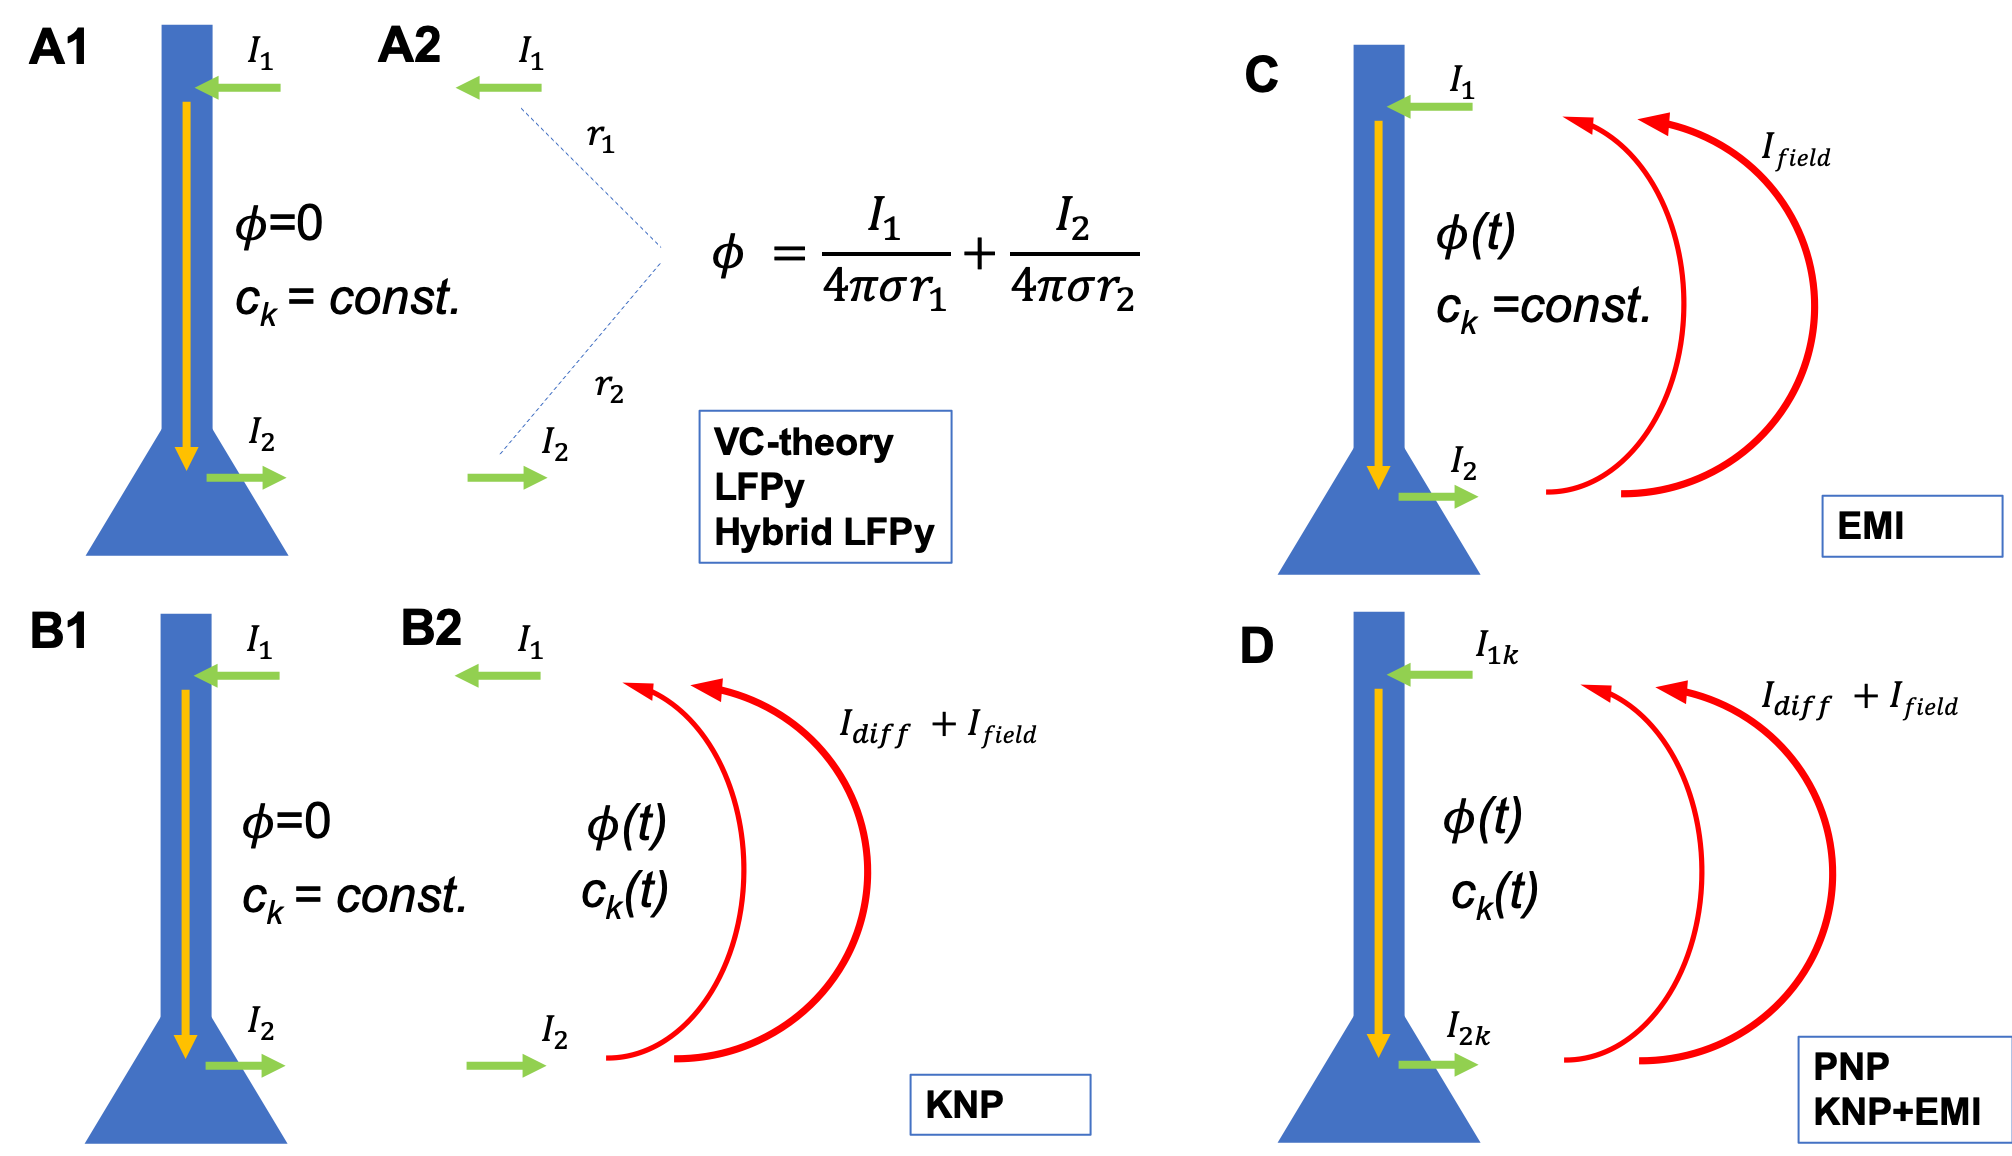
\includegraphics[width=1\textwidth]{Figures/Skjemaoversikt.png}
\end{center}
\caption{\textbf{Overview of the problem that we focus on in this book.} 
}
\label{fig:Knallfigur}
\end{figure}

The simplest take on computing $\phi$ is to treat the extracellular medium as a volume conductor (VC). VC theory then allows us to derive an analytical expression for $\phi$ as a direct function of the neural current sources (Fig. \ref{fig:Knallfigur}A2). Chapter \ref{sec:VC_theory} of this book gives a thorough introduction to VC theory where we derive the key equations from first principles and highlight the many assumptions that the theory is based upon.

A key parameter, and sometimes variable, in VC theory is the conductivity ($\sigma$) of the extracellular medium. In Chapter \ref{sec:conductivity} we give an overview of the experimental and theoretical estimates of $\sigma$. 

Diffusion of ions along extracellular concentration gradients could in principle affect $\phi$. In standard VC theory, such concentrations effects are assumed to be negligible, and ion concentration dynamics is not modeled. This is probably a fairly good approximation for many scenarios, but not for pathological cases, such as epilepsy or spreading depression, which are associated with dramatic concentration shifts in the extracellular medium \cite{Somjen2001, Frohlich2008, Zandt2015review, Ayata2015}. To account for diffusive effects, we need to compute the extracellular dynamics of all individual ion concentrations $c_k$ as well as $\phi$ at all points in space using a suitable numerical electrodiffusive scheme which accounts for diffusion as well as electrical drift og ions (red arrows in Fig. \ref{fig:Knallfigur}B2). In Chapter \ref{sec:eldiff} we present the theory for electrodiffusive processes, and make some estimates of their impact on $\phi$ in different physiological scenarios. 

Another assumption that is typically used when applying VC theory is that the extracellular potential $\phi$ does not have any (ephaptic) effect on the neuronal membrane potential dynamics. This simplifies computations dramatically, because it allows us to perform them in a two-step procedure where we (i) first compute the neurodynamics independently, typically under the assumption that the extracellular potential is zero ($\phi = 0$), and (ii) next use the analytical VC-expression to compute a nonzero $\phi$. The motivation for using this evidently inconsistent approach is that $\phi$ is typically so much smaller than the membrane potential that the ephaptic effects can be neglected without any severe loss in accuracy. This might not be true for all biologically relevant geometries and scenarios, and frameworks that compute the extracellular, membrane and intracellular potentials in a self consistent manner exist (all arrows in Fig. \ref{fig:Knallfigur}C), as do unified frameworks that compute both ion concentrations and electrical potentials in a self consistent manner (all arrows in Fig. \ref{fig:Knallfigur}D). A summary of available frameworks for computing extracellular potentials (and ion concentrations) is given in Chapter \ref{sec:schemes}.

Among the four types of schemes depicted in Fig. \ref{fig:Knallfigur}, the VC scheme is (Fig. \ref{fig:Knallfigur}A) is by far most computationally efficient, as the other schemes require numerical simulations of extracellular dynamics using finite element or finite difference methods. For that reason, the VC scheme is still the gold standard for computing extracellular potentials in large population models of neurons mimicking physiologically realistic scenarios. Therefore, the simulations in the application part of this book (Part 2) will predominantly be based on on standard VC-theory.
